\chapter{RSCP-iBGP系统的设计实现}
\label{cha:design}

\section{本章引言}
本文基于软件路由器Quagga\cite{quagga}的开源代码,实现了RSCP-iBGP内部域间路由协议系统。该系统主要分三部分:边界路由器Route-Client、集中式的路由控制平台上运行的Route-Server、边界路由器与Route-Server之间的扩展iBGP通信协议。本章首先解释设计实现平台Quagga的概念以及其虚拟软件路由器上BGP的路由功能实现细节,之后详细介绍RSCP-iBGP系统的三个部分边界路由器、路由控制平台、通信接口的具体设计与实现。

\section{设计实现平台Quagga介绍}

\begin{figure}
  \centering
  % Requires \usepackage{graphicx}
  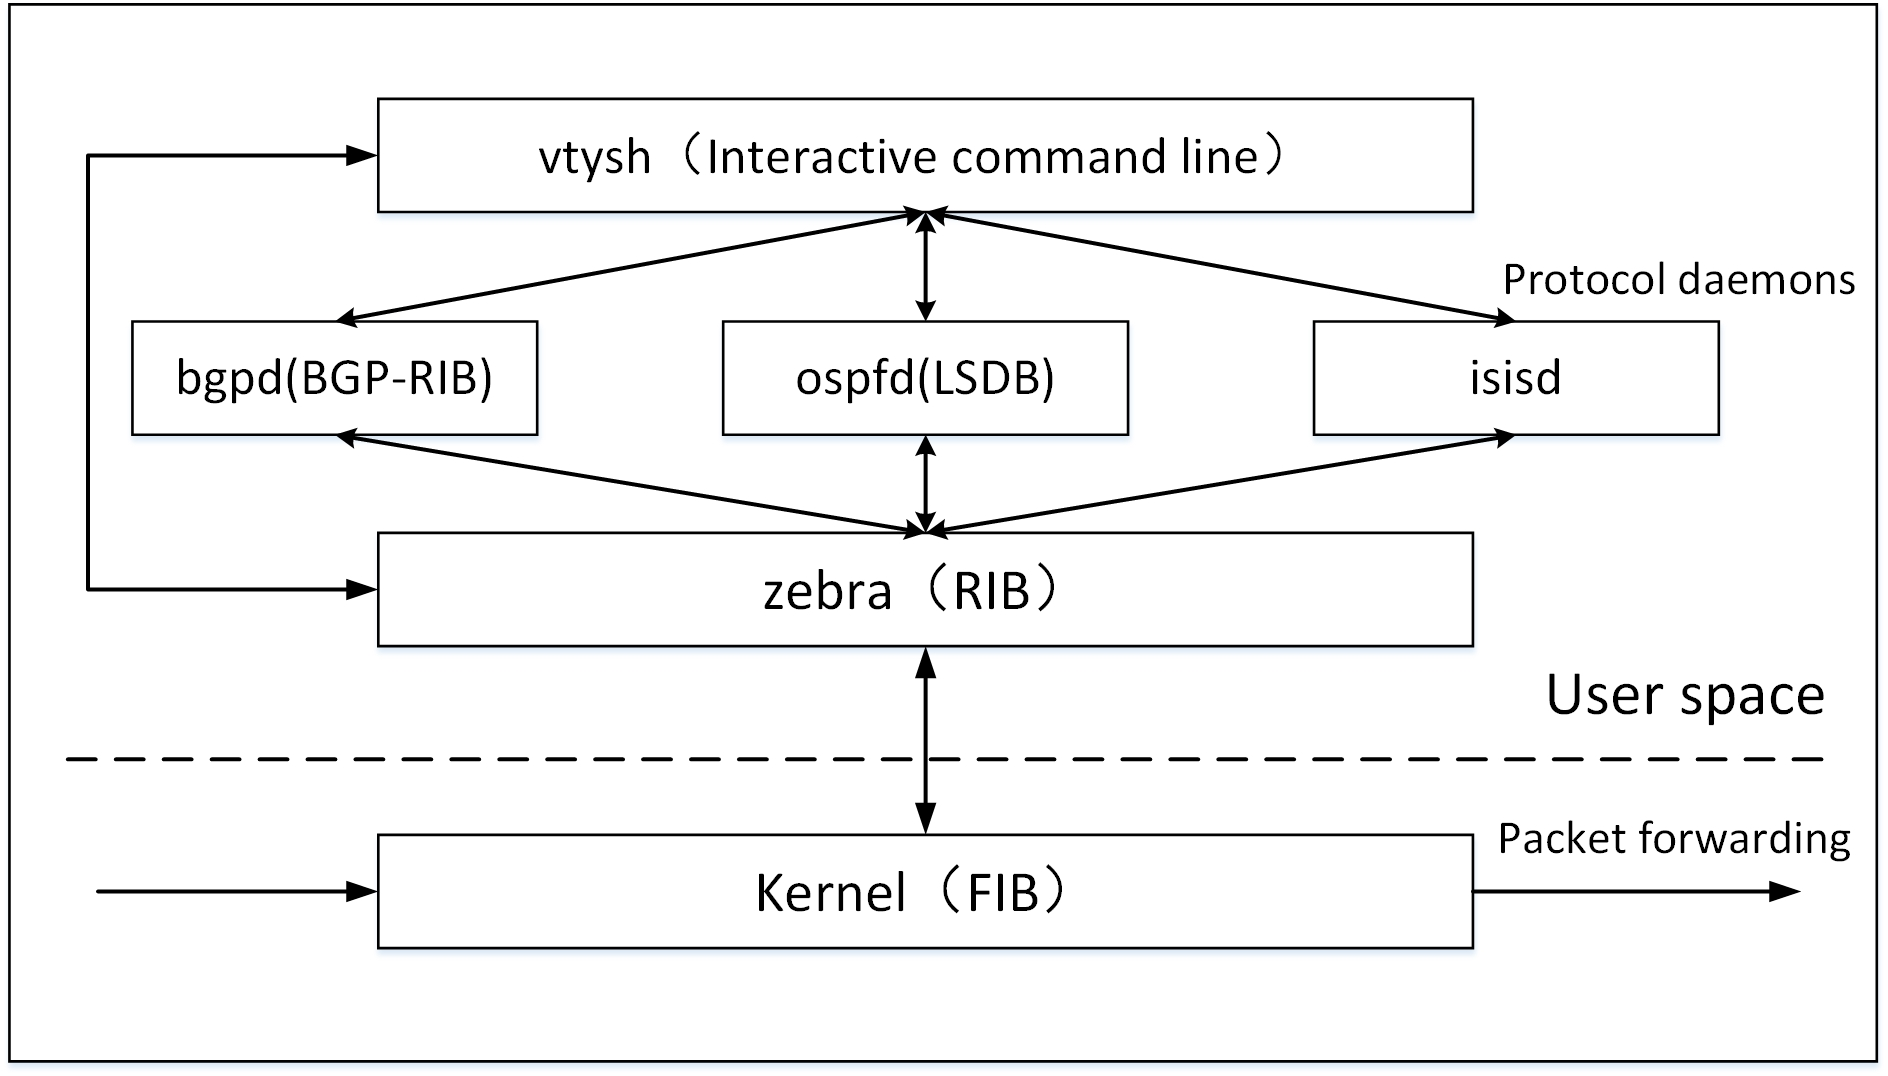
\includegraphics[width=0.75\textwidth]{quagga}
  \caption{Quagga系统结构图\cite{jakma2014quagga}}
  \label{fig:quagga}
\end{figure}


\subsection{基本概念及系统结构}
Quagga是一个比较成熟的虚拟路由器系统,该系统实现了多种网络协议,比如RIPv1、RIPv2、RIPng、OSPFv2、OSPFv3、BGPv4+、IS-IS等。Quagga中不同的网络协议需要运行不同的进程,属于多进程结构,协议之间相互独立,其本身的扩展性、维护性较强 \cite{quaggaThesis}。此外,Quagga中包含一个路由信息管理进程zebra,该进程和各种运行网络协议的进程通过ZServ协议进行交互,将运行网络协议进程产生的有效路由信息安装到内核\cite{jakma2014quagga}。每个协议进程均有自己的配置文件和终端接口,配置不同的网络需要在不同的网络进程内的配置文件中完成,非常麻烦。比如配置BGP网络时,需要在bgpd进程中的配置文件中完成;配置静态路由时,需要在zebra进程中的配置文件中完成。为此,Quagga存在vtysh进程来对Quagga中的其他进程进行配置。vtysh提供一个交互式的命令行接口来输入配置信息,其和其他进程通信通过一个简单的字符串传输协议。在vtysh进程中可以完成网络协议的配置、静态路由配置等对其余每一个进程的配置操作。Quagga的结构如图\ref{fig:quagga}。
\subsection{BGP协议的路由存储}

BGP协议中路由信息表有3种Adj-RIBs-In、Loc-RIB、Adj-RIBs-Out,Quagga中BGP协议的实现在bgpd进程中。bgpd进程中所有的数据结构均存储在bgp\_master结构体中,bgp\_master的成员变量中存在一个链表,包含了所有的bgp实例。每个bgp实例中存储了该BGP session的配置文件、一个链表包含所有的peer实例、静态路由表、路由表(Loc-RIB,结构体为bgp\_table)等信息。


\begin{figure}
  \centering
  % Requires \usepackage{graphicx}
  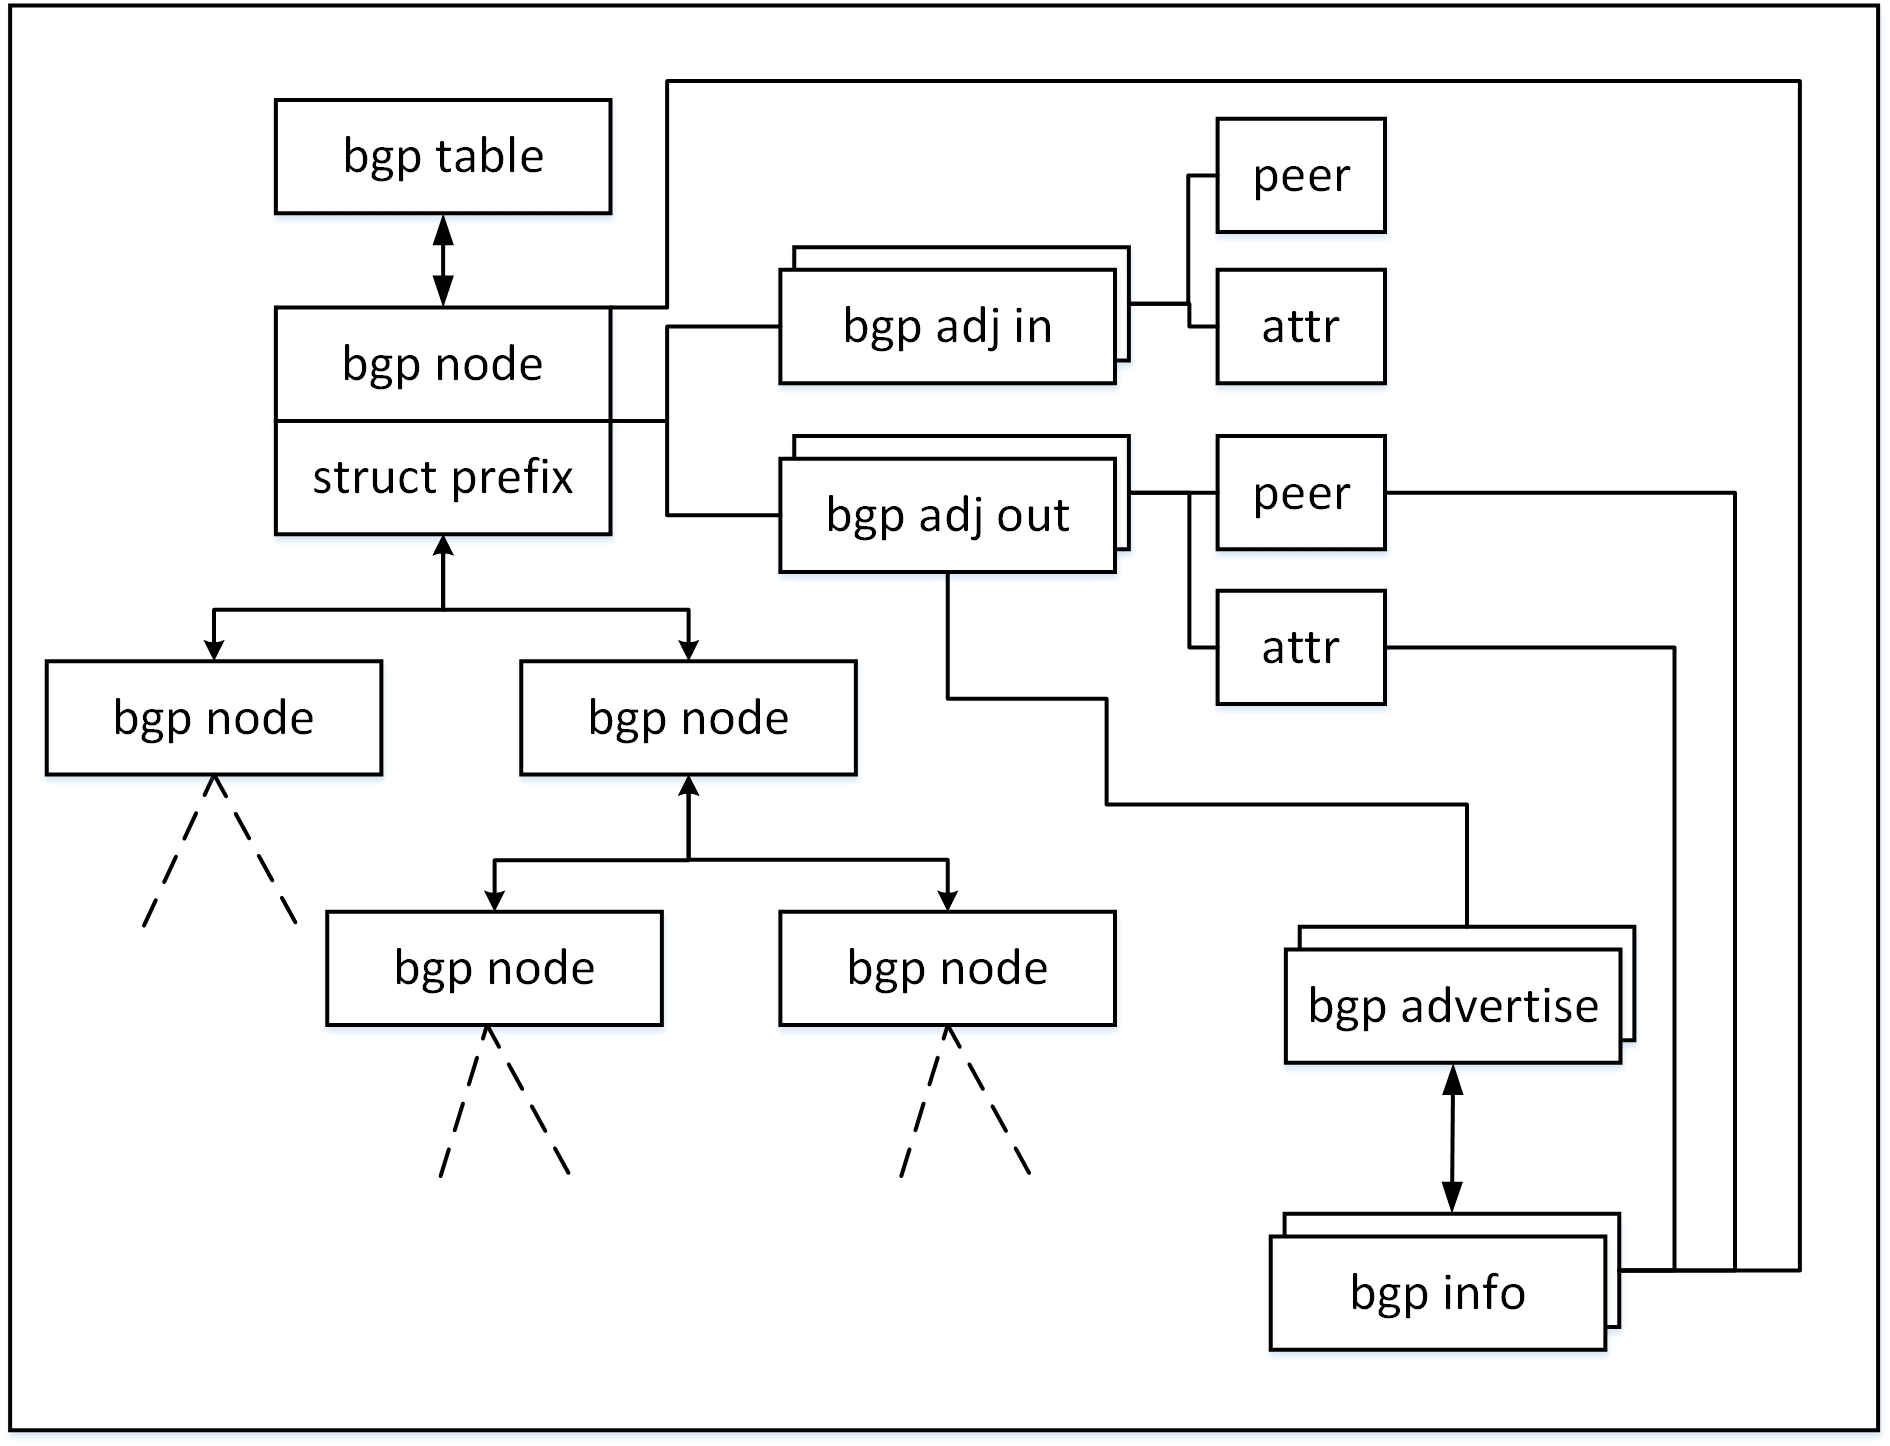
\includegraphics[width=0.75\textwidth]{storage}
  \caption{Quagga-bgpd:BGP路由表概括图\cite{jakma2014quagga}}
  \label{fig:storage}
\end{figure}

Quagga中路由表的存储使用radix二叉树\cite{quaggaThesis}存储结构,radix树是以二进制表示的键值作为树的节点,每个节点通过比较比特位来进行查找,radix二叉搜索树适合处理非常长的,可变长度的键值。每张Loc-RIB表存储在bgp\_table的结构体中,bgp\_table结构体有一个成员变量为bgp\_node类的结构体指针,该结构体指针是该Loc-RIB表radix树结构的根节点,所有路由表项的查找、删除等操作都从该根节点开始。bgp\_node结构体的实例代表的是某前缀所有的路由信息(每一条路由信息用bgp\_info结构体对应的实例表示),bgp\_node结构体中也存在指向bgp\_adj\_in和bgp\_adj\_out的指针。路由信息在bgp\_adj\_in和bgp\_adj\_out中的主要体现是通过他们的成员变量peer和attr。当BGP的某个邻居与之断开连接,则可以通过peer找到对应的prefix,清除bgp\_adj\_in且更新Loc-RIB。

当运行Quagga的虚拟路由器收到路有更新时,如果开启了Adj-RIBs-In存储设置,则会先根据前缀找到对应的bgp\_node,之后根据bgp\_node找到对应的adj\_rib\_in,对其进行更新。当BGP控制台需要输出某对等体的Adj-RIB-In表,则遍历所有的bgp\_node节点,根据bgp\_node找到每条前缀对应的adj\_rib\_in表,遍历该adj\_rib\_in表,如果某路由信息从该对等体收到的,则输出对应的路由信息。

针对某条路由信息bgp\_info向外进行路由宣告时,如果开启了Adj-RIBs-Out存储设置,则会先根据bgp\_info结构体中bgp\_node的指针,找到对应的bgp\_node,之后根据bgp\_node找到对应的adj\_rib\_out,对其进行更新。当BGP控制台需要输出某对等体的Adj-RIB-Out表,则遍历所有的bgp\_node节点,根据bgp\_node找到每条前缀对应的adj\_rib\_out表,遍历该adj\_rib\_out表,如果某路由信息从该对等体宣告出去,则输出对应的路由信息。

综合以上的文字解释,Quagga中实现BGP三张表的存储结构如图\ref{fig:storage}。
\subsection{路由更新流程}

\begin{figure}
  \centering
  % Requires \usepackage{graphicx}
  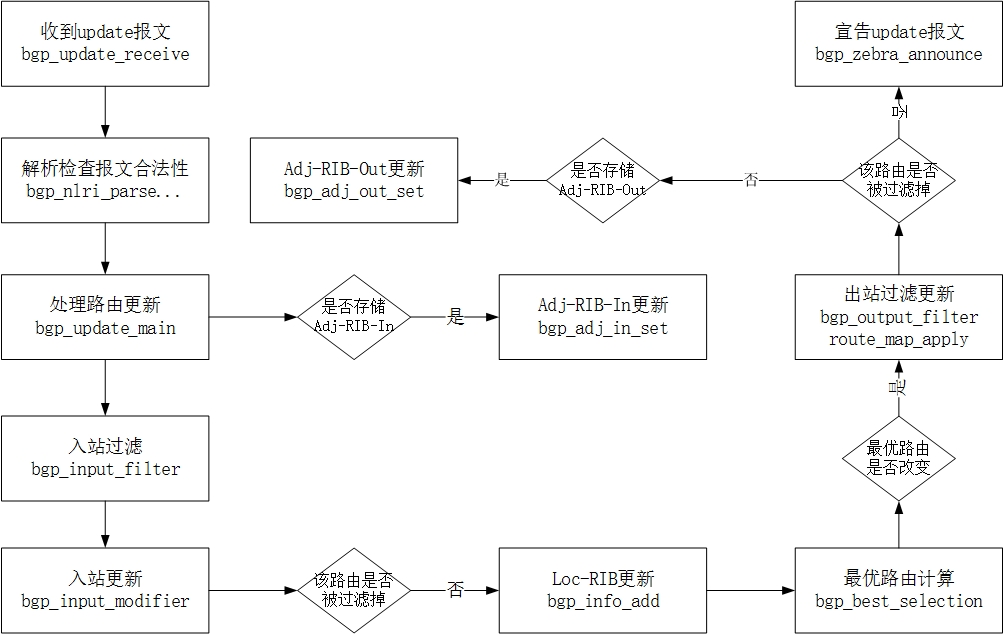
\includegraphics[width=0.8\textwidth]{route-update}
  \caption{Quagga-bgpd:BGP路由更新流程图}
  \label{fig:route-update}
\end{figure}



路由更新过程是虚拟路由器进行路由处理流程的主要部分,对应到Quagga中bgpd进程实现,路由更新的流程如图\ref{fig:route-update}:
\begin{itemize}
  \item 运行Quagga的虚拟路由器先通过bgp\_establish函数与对等体peer建立连接;
  \item 运行Quagga的虚拟路由器通过bgp\_read接收来自对等体的消息;
  \item 当收到BGP消息,通过检查头部的报文格式分析报文类型,如果是UPDATE报文,执行路由更新处理函数bgp\_update\_receive,进行UPDATE报文解析bgp\_nlri\_parse;
  \item 报文解析结束后,执行bgp\_update、bgp\_update\_main等函数进入路由更新消息的处理;
  \item 路由更新消息处理的过程中:如果需要存储Adj-RIBs-In表,进入bgp\_adj\_in\_set函数存储未经过滤的路由信息;之后执行入站过滤bgp\_input\_filter、入站更新bgp\_input\_modifier;如果更新路由没有被过滤掉,则将更新路由其通过info\_make函数生成bgp\_info信息;通过bgp\_info\_add函数将bgp\_info结构体的信息加入Loc\_RIB表中,然后将其通过bgp\_process函数将该bgp\_info路由信息的处理流程加入bgp\_process\_queue队列,该队列使用先进先出的策略;
  \item 当轮到该路由信息bgp\_info处理程序时,进入bgp\_process\_main函数,执行最优路由计算bgp\_best\_selection;
  \item 如果该前缀对应的最优路由发生改变,则执行bgp\_process\_announce\_selected函数,在该函数中有出站过滤更新bgp\_announce\_check和Adj-RIBs-Out更新bgp\_adj\_out\_set;
  \item 最终通过bgp\_zebra\_announce函数将BGP路由向外宣告,且将该最优路由信息注入到RIB表中。
\end{itemize}

\subsection{路由算法}


\begin{figure}
  \centering
  % Requires \usepackage{graphicx}
  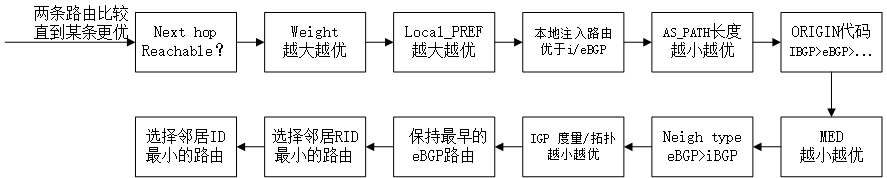
\includegraphics[width=0.9\textwidth]{route-cmp}
  \caption{Quagga-bgpd:BGP路由比较步骤}
  \label{fig:route-cmp}
\end{figure}

Quagga的bgpd进程中路由算法主要是在bgp\_best\_selection函数中实现的。针对前缀Prefix,在bgp\_table中找到该前缀对应的所有路由信息bgp\_node。路由信息的存储使用链表的数据结构,最新的路由会插在表头,所以bgp\_node存储的同一前缀的路由信息是按照更新时间由近及远进行存储。将该前缀对应的路由信息由近及远两两通过bgp\_info\_cmp进行比较,得到前缀的最优路由。两两比较选更优,比较步骤如图\ref{fig:route-cmp}。


\section{系统设计与实现}
每个网元内部的协议报文处理流程


\subsection{边界路由器}
边界路由器Route-Client收到集中平台Route-Server通过iBGP协议发来的最优路由,最优路由将会被提交到IP路由表中,相同前缀下拥有最低AD值的路由协议提交的最优路由最终会被放入IP路由表中,当路由器收到数据包时,通过IP路由表进行转发\cite{DianeTeare2016CCNP}。

当边界路由器Route-Client收到eBGP路由时,将经过入站策略的eBGP路由信息通过扩展的iBGP协议,直接传输给集中平台上的Route-Server。
当边界路由器Route-Client收到iBGP路由时,经过出站策略的路由信息宣告给所有的eBGP邻居。


\subsection{路由控制平台}
\subsubsection{路由存储}
\subsubsection{路由计算}
具体实现方法和算法分析
路由算法的伪代码

\subsection{通信接口}
通信接口通过扩展的iBGP协议进行实现,边界路由器Route-Client需要发送携带Weight路径属性的UPDATE报文信息到集中平台Route-Server,且Route-Server收到扩展iBGP协议发来的携带Weight路径属性的UPDATE报文需要能够进行正常识别和解析。

边界路由器上运行的BGP协议需要在给邻居发送UPDATE报文的时候携带Weight路径属性,所以在边界路由器上运行的软件路由器Quagga中,需要修改UPDATE报文的Path Attributes部分,增加传输Weight路径属性。在Quagga中的BGP协议代码实现UPDATE报文中,Path Attributes的组包实现函数为bgp\_packet\_attribute(bgpd\_attr.c文件中),在其他属性添加结束后,在字节流后添加Path Attribute的三元组。传输Weight属性的三元组中,Flag=0x40和Type Code=0x1f,Length=0x02,Value值长度为2个字节。如果传输的Weight值为150,则对应的传输Weight的Path  Attribute为0x401f020096。

\lstset{language=C}
\begin{lstlisting}
//s is Path Attributes Stream;
//#define BGP_ATTR_FLAG_TRANS     0x40
//#define BGP_ATTR_WEIGHT         31
stream_putc (s, BGP_ATTR_FLAG_TRANS);
stream_putc (s, BGP_ATTR_WEIGHT);
stream_putc (s, 2);
stream_putw (s, attr->extra->weight);
\end{lstlisting}


集中平台上Route-Server收到携带Weight路径属性值的UPDATE报文后,需要对齐进行正确的解析。Quagga中的BGP协议代码实现Path Attributes解析的函数为bgp\_attr\_parse(bgpd\_attr.c文件中),根据Type Code执行不同的Path Attribute解析函数,Weight属性的解析函数需要检查Length是否为2。如果不为2,需要执行bgp\_notify\_send函数,回复对等体NOTIFICATION报错(Path Attribute长度错误)。



\section{本章小结}
本章对SRCP-iBGP系统的实现平台Quagga进行了详细的介绍,了解虚拟路由器的BGP路由实现之后,更容易理解本文提出的SRCP-iBGP系统的设计与实现。
